\chapter[Revisiting the punctuated equilibrium debate in light of emerging phylogenetic data and methods]{Revisiting the punctuated equilibrium debate in light of emerging phylogenetic data and methods\footnote{Previously published as: Pennell M.W., Harmon L.J., and Uyeda J.C. 2014.
  Is there room for punctuated equilibrium in macroevolution?
  Trends in Ecology \& Evolution 29:23--32}}
\label{chap:punceq}

\section{Summary}

The long-controversial theory of punctuated equlibrium (PE) asserts that speciation causes rapid evolution against a backdrop of stasis. PE is currently undergoing a resurgence driven by new developments in statistical methods. However, we argue that PE is actually a tangle of four unnecessarily conflated questions: i) is evolution gradualistic or pulsed?; ii) does trait evolution occur mainly at speciation or within a lineage?; iii) are changes at speciation adaptive or neutral?; and iv) how important is species selection in shaping patterns of diversity? We discuss progress towards answering these four questions but argue that combining these conceptually distinct ideas under the single framework of PE is distracting and confusing, and more likely to hinder progress than to spur it.


\section{Introduction: the resurgence of punctuated equilibrium}

The following three quotations were all drawn from abstracts of recent papers purporting to use statistical models to empirically evaluate punctuated equilibrium (PE):

\begin{quote}
\singlespacing
A long-standing debate in evolutionary biology concerns whether species diverge gradually through time or by punctuational episodes at the time of speciation. We found that approximately 22\% of substitutional changes at the DNA level can be attributed to punctuational evolution, and the remainder accumulates from background gradual divergence. \citep[][p. 119]{Pagel2006}
\end{quote}

\begin{quote}
\singlespacing
This controversy, widely known as the `punctuated equilibrium' debate, remained unresolved, largely owing to the difficulty of distinguishing biological species from fossil remains. We analyzed body masses of 2143 existing mammal species on a phylogeny comprising 4510 (i.e. nearly all) extant species to estimate rates of gradual (anagenetic) and speciational (cladogenetic) evolution. \citep[][p. 2195]{Mattila2008}
\end{quote}

\begin{quote}
\singlespacing
Under such processes, observations at the tips of a phylogenetic tree have a multivariate Gaussian distribution, which may lead to suboptimal model specification under certain evolutionary conditions, as supposed in models of punctuated equilibrium or adaptive radiation. \citep[][p. 193]{Landis2012}
\end{quote}
These three papers are representative of a substantial number of other recent high-profile studies that have discussed their research in the context of PE \citep[e.g.,][]{Hunt2007, Hunt2008, Huntetal2008, Webster2003, Bokma2002, Bokma2008, Ingram2011, Uyeda2011, Rabosky2012, Hunt2012, Bartoszek2013, Rabosky2013, Simpson2013, Atkinson2008, Baca2013}. This is somewhat remarkable given that arguably no idea has had such a turbulent history in modern evolutionary thought as punctuated equilibrium. In the early 1970s, Eldredge and Gould \citep{Eldredge1971, EldredgeGould1972, GouldEldredge1977} proposed that the predominant pattern of evolution throughout deep time is that of stasis ``punctuated'' by brief intervals of rapid evolution, which often occurred during speciation events. This was originally conceived as a way of bridging the gap between prevailing ideas about speciation, i.e., Mayr's allopatric model \citeyearpar{Mayr}, and observations from the fossil record \citep{Sepkoskibook}. However, PE has expanded and shifted in definition to become a much more far-reaching hypothesis to many researchers. Consequently, it has been viewed as both a a rather innocuous statement about the general patterns found in the fossil record and as an affront to the central tenets of evolutionary theory \citep{Stanley1975, Stanley1979, Gould1980, Charlesworth1982, Levinton2001}. For some researchers, the stakes of the debate over the prevalence of PE could not have been higher:

\begin{quote}
\singlespacing
If most evolutionary changes occurs during speciation events, and if speciation events are largely random, natural selection, long viewed as the process guiding evolutionary change, cannot play a significant role in determining the overall course of evolution. Macroevolution is decoupled from microevolution... \citep[][p. 648]{Stanley1975}
\end{quote}

In the wake of such claims, much of the intellectual history of PE was been characterized by fierce, and often vitriolic, theoretical debates--exhaustively catalogued in \citep{Levinton2001, Gould2002}--and the theory remains divisive \citep[for more on the history of the idea, see][]{Sepkoskibook}.

The field of macroevolution has recently witnessed a resurgence of interest in PE as paleobiologists and, increasingly, comparative biologists armed with molecular phylogenies, have applied sophisticated statistical models to quantitatively test the major hypotheses of PE. In this review, we ask whether these new statistical advances have ``rescued'' PE from intellectual extinction. We answer this question in the negative. The challenges inherent in elucidating macroevolutionary processes and patterns from paleontological and comparative data are only exacerbated by the muddled historical legacy of PE. Although a number of studies have indeed discussed their findings in light of PE, they have actually addressed a wide variety of conceptual issues; the studies from which we have quoted above exemplify this--each one asks a fundamentally distinct question.

What then, exactly, defines PE? The central definitions and concepts of PE have shifted substantially over time--including the views of the theory's chief advocates \citep{Mayr1982, Ruse1989, Sepkoskibook}. We argue that the key to disentangling this Gouldian knot, lies not in attempting to parse the literature in search of the true ``essence'' of PE, but rather in recognizing that the myriad concepts often associated with the theory can be conceptually dissociated and evaluated independently. We believe that dissociating the different components of PE will lead to a more productive discussion of these ideas and facilitate progress in some of the most fundamental questions in macroevolution. In this essay, we identify four key questions that have been lumped under the topic of PE, discuss how their association with each other has led to confusion, and comment on recent methodological developments, using a variety of types of data, that may provide novel insights into large-scale patterns of diversity.

\section{Punctuated equilibrium as a conglomerate of concepts}

In our view, the theory of PE, and the extensive discussion surrounding it, conflates four separate primary research questions: i) what is the relative importance of gradualistic versus pulsed evolution?; ii) what is the role of speciational events (cladogenesis) vesus within lineage evolution (anagensis) in generating trait divergence?; iii) when change is cladogenetic, are these changes adaptive or driven by neutral processes?; and iv) how important is higher level selection (species selection) in shaping patterns of diversity? 

\subsection{Gradualistic versus pulsed evolution}

In principle, it is quite feasible to distinguish gradualistic versus pulsed evolution using either phylogenetic comparative or paleontological data. Constant-rate gradualism is typically modeled as a random walk or Brownian motion process in both phylogenetic and paleobiological studies (BM; see \textsc{box 1}). Several recent studies have examined whether fossil time-series conform better to predictions from constant-rate BM, phenotypic stasis, or directional evolution, which each predict different distributions of trait values through time and can be distinguished using model selection techniques \citep{Hunt2012}. These studies have found mixed support for each mode of evolution in different lineages and traits \citep{Hunt2007, Huntetal2008, Hunt2008, Grey2008, Hopkins2012, Hunt2012}. An exceptional demonstration of pulsed evolution in the fossil record was examined by \citet{Huntetal2008}, who found support for a rapid pulse of evolution in sticklebacks as they colonized a novel adaptive peak. Similar model-fitting approaches have been used to demonstrate that in particular fossil time-series shifts in the mode of evolution (i.e., directional evolution, stasis, or BM) are separated by phenotypic bursts \citep{Hunt2008}. This pulsed pattern of evolution is supported by large collections of micro- and macroevolutionary data \citep{EstesArnold2007, Uyeda2011}. Studies of fossil time-series often include a number of caveats that may complicate inference of evolutionary modes. These include unequal sampling probabilities and uncertain stratigraphic position, as well as issues relating to range shifts, time-averaging and phenotypic plasticity \citep{StratPaleobook}. A particularly promising, albeit data-intensive, method developed by \citet{Hannisdal2007} incorporates some of these additional sources of uncertainty in a Bayesian framework.

While fossil time-series provide direct observations of phenotypes over time, they are limited by the difficulty in confidently assembling sequences of ancestor-descendant relationships. Phylogenetic comparative methods provide a complementary means to study departures from constant-rate gradualism; these can be applied to both extant and extinct data, if the fossil data can be placed in a phylogenetic context \citep{PennellHarmon}. Several methods allow the detection of rate shifts across clades by allowing the BM rate parameter $\sigma^2$ to differ across branches of the phylogeny \citep[e.g.,][]{Omeara2006, Eastman2011, Slater2012MECCA}. However, these methods model sustained shifts in evolutionary rates, rather than pulsed patterns suggested by PE. Pure-burst models, in which all change accumulates in pulses, can also be fit to phylogenies and more closely align with PE \citep{HansenMartins1996, Khaitovich2005, Uyeda2011}. \citet{Landis2012} developed a particularly promising approach that models both gradual and punctuational patterns of evolution using jump-diffusion models, in which both jumps and gradual evolution come from a single, long-tailed distribution \citep[see also,][]{Eastmanjump}. In addition to these methods, discrete shifts in adaptive optima separated by long periods of stabilizing selection have been extensively implemented in in phylogenetic comparative methods by using Ornstein-Uhlenbeck (OU) models \citep{Felsenstein1988, Hansen1997, ButlerKing2004}. OU models are attractive alternatives to BM that can incorporate stasis, stabilizing selection and adaptive hypotheses \citep[][see \textsc{box 1} for further details]{PennellHarmon}. 

Advances in quantitative model-fitting of evolutionary processes have allowed us to explore much wider range of evolutionary hypotheses and processes than simple BM \citep{PennellHarmon}, including pulsed evolutionary patterns. However, to what extent does the framework of punctuated equilibrium contribute to interpretation of the results of these models? Note that none of the models described in this section can distinguish between cladogenetic or anagenetic change (see next section). Furthermore, PE is tied to a very specific pattern of evolution and a specific temporal frame: stasis over the lifespan of a species (typically millions of years) followed by geologically brief bursts of phenotypic evolution occurring at speciation \citep{EldredgeGould1972, GouldEldredge1977, Gould2002}.  Therefore, even robust support for a pattern of pulsed evolution--represented by shifts in trait values along branches that are not accounted for by gradual evolution--may be incompatible with PE if the pulses occur too infrequently for conventional PE theory, which predicts pulses at all (or nearly all) speciation events. In addition, exactly as paleontologists have long recognized that repeated burst-stasis episodes can appear gradualistic if viewed at too coarse a scale, gradualistic evolution with variable rates can appear pulse-like at the same coarse scale. A pulsed pattern detected from phylogenies--which typically have much longer timescales and coarser sampling than a fossil time-series, may not reflect phenotypic bursts between species. Instead, model-fits may reflect ``jumps'' between higher-level niche space or adaptive zones, within which whole clades or groups of species may cluster \citep{Simpson1944, Hansen1997, Hansen2012book, Eastmanjump}. The observation that groups of species cluster around different phenotypic optima says nothing about whether individual lineages exhibit a pattern of stasis and phenotypic bursts of evolution over the lifespan of individual species. Tying patterns measured at phylogenetic scales to species-level and not clade-level change is fraught with difficulty. However, we can still address other interesting macroevolutionary questions such as whether evolution is characterized by pulses, how often they occur and what ecological factors may be associated with them \citep{Eastmanjump}.

\subsection{Anagenetic versus cladogenetic change}

Although speciation is undoubtedly associated with genetic and trait divergence \citep[][and references therein]{Nosil2012}, its relative importance compared to evolutionary change within a lineage is currently poorly understood. Several studies have attempted to evaluate the contribution of cladogenetic change to trait evolution \citep{WagnerErwin1995, JC1999, Aze2011, Strotz2013} using paleontological data. This is evaluated by determining whether the stratigraphic ranges of descendant species overlap with their progenitor species, indicative of coexistence and cladogenesis. However, robustly distinguishing between cladogenetic and anagenetic changes using fossil data crucially depends on several assumptions, such as the accurate reconstruction of ancestor-descendant relationships, the equivalency of species concepts applied to fossil and extant taxa, the robust estimation of species' temporal ranges and enough sampling to eliminate the possibility of gradual evolution \citep{JC1999}. Disputes over the validity of these assumptions have been well played out in the punctuated equilibrium literature \citep[e.g., the Turkana Basin molluscs,][]{Williamson1981, Fryer1983, VanBocxlaer2008}. Approaches have been developed to account for potential biases, such as estimating ancestor-descendant relationships \citep{Marshall1995, Foote1996} and stratigraphic ranges \citep{Marshall1990, Marshall1994, Marshall1997, Wagner2000}, accounting for sampling, but difficulties remain.  As a recent example, \citet{Strotz2013} found a predominance of cladogenetic change among fossil Foraminifera, using assumed ancestor-descendant relationships assembled from stratigraphic and phenotypic data \citep{Aze2011}. We view such claims with considerable skepticism because it is impossible to detect cryptic speciation--which is increasingly being inferred in extant groups \citep{Fujita2012}--in the fossil record, and therefore distinguish decisively between anagenetic and cladogenetic change.

Another tactic to assess the relative contributions of anagenetic and cladogenetic change has been to look for correlations between speciation rates (or species richness, as a proxy for speciation rates) and rates of evolution using phylogenetic comparative data. This has been done by fitting regression models between inferred lineage-specific rates of evolution and diversification. Several studies have demonstrated such a correlation using a variety of characters, including genetic changes \citep{Webster2003, Pagel2006, VendittiPagel2010}, morphological traits \citep{Ricklefs2004, Adams2009, RaboskyAdams2012, Rabosky2013} and linguistic characters \citep{Atkinson2008}. However, demonstrating a correlation between speciation rates and trait evolution does not demonstrate that the actual speciation events themselves are associated with evolutionary change. For example, higher rates of speciation and trait evolution might both be driven by a common cause \citep[][see below, \textsc{box 2},]{Rabosky2012}.

A more promising avenue for partitioning out the influence of cladogenetic versus anagenetic change is to use statistical models, which explicitly parameterize both of these components and simultaneously estimate them using maximum likelihood or Bayesian inference. Early forms of such models assumed that all speciation events were captured by the reconstructed phylogeny. These methods partition the variance in trait values between the speciation events and the background evolution occurring within a lineage \citep{Pagel1997, Mooers1999, Bokma2002, Wagner2000, WagnerMarcot2010}. More sophisticated approaches attempt to simultaneously model the diversification process together with trait evolution \citep[][see \textsc{box 3} for details]{Bokma2002, Mattila2008, Bokma2008, Bokma2010, Goldberg2012, MagnusonFord2012, Simpson2013} to account for the fact that extinction has erased many of the speciation events in the inferred phylogeny \citep{Nee1992, Nee1994, Nee2006, Ricklefs2007}. Such model-based approaches are not without caveats. Importantly, violations of simplifying assumptions may strongly affect inferences, and methods to evaluate model adequacy are sorely needed. Furthermore, unaccounted measurement error may be erroneously folded into estimates of cladogenetic change. In fact, we should expect samples of recently diverged species to differ substantially regardless of whether evolution is punctuational or gradual--even after accounting for simple forms of sampling error--due to within-lineage processes \citep[e.g., as the result of geographic range variation;][]{Uyeda2011, Houle2011, Hansen2012book}. These processes may or may not be important for macroevolutionary patterns, and are difficult to model using current comparative methods \citep{Futuyma1987,Futuyma2010,Stone2011}.
	
Even when speciation is inferred to be associated with divergence, a broader conceptual issue remains: what are the causal mechanisms that could generate such an association against a general backdrop of apparent stasis \citep{BentonPearson2001, Eldredge2005}? Speciation has long been thought of as a major driver of phenotypic change, both in the context of PE and in evolutionary biology more broadly \citep{Saetre2013}. In their original conception of PE, Eldredge and Gould \citep{Eldredge1971, EldredgeGould1972} viewed the pattern posited by PE as a consequence of Mayr's model of allopatric speciation \citep{Mayr}; as such, speciation is considered a mechanism that interrupts stasis \citep{Futuyma1987, Futuyma2010}. However, the causes of stasis in macroevolutionary data are still unclear \citep{Futuyma2010, HansenHoule2004, EstesArnold2007, WalshBlows2009}. In particular, the direction of causality cannot be elucidated from the statistical methods we have described. Alternative explanations remain such that trait evolution often generates reproductively isolated lineages or that both species diversification and trait evolution rates increase with greater evolutionary ``versatility'' or ``evolvability'' \citep{Vermeij1973, Adamowicz2008, Rabosky2013}. There is some evidence that there is variation in the ability of lineages to evolve novel phenotypes \citep{Liem1975, Martin2011} though the causes of this variation are still poorly understood are deserve further research.  Regardless, it is important to recognize that a central tenet of PE theory--that speciation causally leads to phenotypic evolution--remains impossible to evaluate from either phylogenetic comparative or paleontological data. 

\subsection{Adaptive versus neutral evolution at speciation}

One of the most contentious ideas surrounding PE is that changes associated with speciation are random or neutral; this is what led Gould, Stanley and others to claim that macro- and microevolution were effectively ``decoupled''. There are actually two specific versions of this question and these, similarly to many of the ideas we discuss throughout the paper, have often been conflated. The first version is that the changes that occur are random with respect to the direction of a macroevolutionary trend. This is referred to as ``Wright's rule'' in the paleobiology literature \citep{GouldEldredge1977} and has been evaluated by testing whether trait differences between ancestors and descendants are directionally biased by evaluating whether the mean of the distribution of changes in significantly different than zero, the null expectation under most models of trait evolution \citep{Wagner1996, Wagner2001}. For example, if there is a trend of increasing body size throughout the history of a clade (Cope's rule), then Wright's rule requires that daughter species, at speciation, are on average no bigger (or smaller) than their ancestor. To Gould and Eldredge \citeyearpar{GouldEldredge1977}, as well as to other researchers \citep[for example,][]{Stanley1975, Stanley1979}, Wright's rule was a key justification for including species selection in a PE framework; if change only occurs at speciation and that change is random with respect to macroevolutionary trends, those trends can only be explained by species selection. However, if we recognize that the nature of change at speciation is independent of species selection (see below), then establishing Wright's rule has no bearing on the strength of higher level selection \citep{Simpson2013}. At the same time, biased transmission may still be involved in macroevolutionary trends \citep{Wagner1996, McShea1994, McShea1998}.

The second, broader version of the claim is that change at speciation is driven by neutral processes rather than adaptive evolution \citep{Stanley1979, Gould1980, Gould2002}. This is much more complex to address. There have been several attempts to investigate the hypothesis that past trait changes were adaptive using phylogenetic comparative or paleobiological data  \citep[see for example,][]{Adaptation}. For example, phylogenetic methods can attempt to associate trait changes with changes in the selective regimes experienced by those lineages \citep{Baum1991, ButlerKing2004, Beaulieu2012}, or studies of functional morphology can provide specific hypotheses about relationships between trait states and the environment, which can then be tested statistically \citep{Wainwright2007}. However, these necessarily rely on either detailed information about form, function, and the environment \citep[e.g.,][and references therein]{Vermeij1987} or researcher's a priori hypotheses regarding what was adaptive at some period in the past. We know from studies of wild populations that the direction of selection is often temporally and spatially variable \citep{Grant2002, Siepielski2009, Siepielski2011} and it is therefore extremely tenuous to draw conclusions regarding the adaptive value of changes during speciation from comparative or paleontological data alone.

There has been a great deal of study investigating the patterns of evolution throughout the course of speciation using natural populations, experimental systems and mathematical models \citep[][and references within]{Schluter2000, CoyneOrr, Gavrilets2004, Rundle2005, Doebeli2011, Nosil2012}.  In particular, many recent studies have explored the distinction between ecological speciation, where speciation is driven by divergent natural selection between lineages, and other forms of speciation \citep[e.g., Bateson-Dobzhansky-Muller incompatibilities, speciation driven by sexual selection, etc.; reviewed in ][]{Nosil2012}. As a result of these studies, we have learned a great deal about the mechanisms involved in speciation and are beginning to understand the relative importance of adaptive and neutral processes during speciation across a broad suite of taxa--although it is much too early to draw any sweeping conclusions. We strongly suggest that this avenue of research is far more appropriate for addressing this aspect of PE than analyzing either phylogenetic comparative or paleontological data alone. 

\subsection{Species selection as a macroevolutionary process}

Though long controversial in its own right \citep{FitzJohnthesis}, the idea that natural selection can act on species-level characteristics is becoming more widely appreciated \citep{CoyneOrr, Jablonski2008, RaboskyMcCune2010, FitzJohnthesis}. Here we follow the lead of other authors \citep{Williams1992, CoyneOrr, RaboskyMcCune2010} and define species selection as  ``repeatable effects of that trait on the rate of diversification of species possessing it'' \citep[][p. 444]{CoyneOrr}, regardless of whether or not the trait is an emergent property of the lineage or the aggregate of individual-level traits. We therefore ignore the (in our view, unnecessary) distinction between ``species selection'' and ``species sorting'' \citep[\textit{sensu}][]{GouldVrba1986} For an alternative perspective on this issue, see Jablonski's excellent review \citeyearpar{Jablonski2008} of the topic.

The idea that the tempo and mode of evolutionary change is inexorably linked to selection at the lineage level is an old and persistent one and is, in the minds of at least some researchers, part and parcel of a broader macroevolutionary theory \citep{Stanley1975, Stanley1979, GouldEldredge1977, Gould1980, Charlesworth1982, Dennett1995, Levinton2001, Gould2002}. The reasoning behind this is that, in some researcher's conception of the process, selection can only act on ``evolutionary individuals'' \citep{Hull1980} and species can only operate as such if they have a definite beginning and end \citep{GouldEldredge1977, Gould2002}--a pattern that is produced if evolutionary change only occurs at cladogenesis. Although this may seem intuitive, such an association is logically (and mathematically) unnecessary. Species selection does not require any particular mode of evolutionary change and it certainly does not require the majority of change to be concentrated at speciational events \citep{VanValen1975, Bookstein1978, Slatkin1981, ArnoldFristrup1982, Rice1995, McShea2004, Rice2004, Okasha2006, Jablonski2008, Simpson2013}. The conflation of species selection with punctuated change has been cited by some authors to be a cause of antagonism towards species selection \citep{Turner2010, FitzJohnthesis}.

Species selection has been recently reviewed in depth \citep{Jablonski2008, RaboskyMcCune2010} and we will not attempt to be comprehensive here. Instead, we focus on recent methodological developments that have improved our ability to detect species selection. Conventionally, inference regarding the influence of a trait on diversification rate from molecular phylogenies has been carried out by comparing the diversities or diversification rate between independent pairs of sister taxa \citep{Mitter1988, Sargent2004, Vamosi2004, RaboskyMcCune2010}. However, this is problematic for several reasons including statistical power \citep{Slowinski1989, Slowinski1993, VamosiVamosi} and that asymmetries in character transition rates can confound asymmetries in diversification rate (and \emph{vise versa}) \citep{Maddison2006}. A major innovation to simultaneously deal with this issue and investigate the correlation between traits and speciation and extinction was made by \citet{Maddison2007}, with their Binary State Speciation and Extinction, or \textsc{bisse}, model (see \textsc{box 3}). This has been extended beyond binary traits to investigate the effect of multiple discrete traits \citep[\textsc{musse};][]{FitzJohn2012}, quantitative traits \citep[\textsc{quasse};][]{FitzJohn2010} and geographic range \citep[\textsc{geosse};][]{Goldberg2011} on lineage diversification. We note that although these are certainly very promising statistical approaches, they rely on some large sample sizes and potentially dubious assumptions, such as that diversification can be modeled as constant-rate branching process \citep[i.e., a ``birth-death'' model;][]{Kendall1948}, that rates of evolution are constant across the phylogeny, and that the directionality and strength of species selection is consistent. There is substantial evidence that suggests that diversification rates are not constant through time or across clades \citep{Rabosky2007, McPeek2008, PhillimorePrice2008, Alfaro2009, Rabosky2012, Rabosky2013}, perhaps owing to diversity-dependent diversification \citep{Sepkoski1984, Alroy2008, Rabosky2009}, and this has been a focus of modeling work in both paleobiology \citep{Roy1996,  Eble2000, Sepkoski2000} and phylogenetic comparative methods \citep{Rabosky2008, Etienne2012, Etienne2012AmNat}. Similarly, rates of trait evolution are likely often quite heterogeneous \citep{Eastman2011, Beaulieu2013} and the vector of species selection has been inferred to be variable in some groups \citep{Jablonski1986, Simpson2010, Harnik2012}. Some of these assumptions can potentially be relaxed \citep{RaboskyGlor2010} but in general, the robustness of these methods to severe violations awaits further investigation.

In paleontological research, there has been increasing development of multivariate methods to partition out the effect of various correlated traits on speciation and or extinction, which is key to elucidating causal mechanisms. This has been accomplished using statistical techniques such as general linear models (i.e., predict lineages' diversification rates or durations in the fossil record from lineage-specific traits) \citep{JablonskiHunt2006, Harnik2011, Harnik2012}. Alternatively researchers have used the Price Equation \citep{Price1972, Rice2004, Okasha2006, Frank2012} to examine the covariance between traits and diversification rates. The Price equation was first proposed for the purposes of studying macroevolution by Arnold and Fristrup \citep{ArnoldFristrup1982}, and this has recently been expanded upon by Simpson and colleagues \citep{SimpsonHarnik2009, Simpson2010}. Adopting the Price equation also allows for the possibility of a unified approach to the study of species selection across data-types that could potentially be applied to both phylogenetic comparative data and fossil time-series \citep{Jablonski2008,Simpson2013}. 

\section{Concluding remarks}

In this paper, we have described quantitative approaches to addressing four fundamental macroevolutionary questions that have long been conflated with each other in the literature on PE. Confusion among these disparate and independent questions has led many researchers to consider PE as being robustly verified, whereas others believe the theory bankrupt of empirical support. Either view may be justified depending on which component an individual researcher considers the essence of PE theory. If macroevolutionary researchers dissociate these concepts, the fact that some may be more difficult to evaluate or are less theoretically sound should not impede progress on other questions.

Although we argue throughout that the questions that make up PE can be addressed independently, this does not preclude synthesis. Instead, multiple processes could be important (and often, probably are) to understanding the accumulation of diversity and disparity through deep time. For example, \citet{Goldberg2010} used the \textsc{bisse} model to demonstrate that species selection was important for maintaining self-incompatibility in the plant family Solanaceae (the ``nightshade'' family). In a subsequent paper, \citet{Goldberg2012}, re-analyzed the same data but used a model that allowed for trait evolution within a lineage, species selection, and (additionally) trait evolution occurring at cladogenesis (see \textsc{box 3} for details). They found that all three processes appear to be important in this group. Nonetheless, these are independent processes that may or may not be linked mechanistically, in this group or others.

Instead of bringing new insight into PE--and thereby rescuing the term from its historical problems--novel developments have demonstrated that the terminology associated with PE can be problematic. We believe that emerging statistical models and datasets are best suited for testing independent components of PE theory. Evaluation of these methods in the context of PE will only lead to confusion. Although PE undoubtedly served as a catalyst in the development of concepts and methods discussed above, we think it is time to move on, and encourage researchers in macroevolution to look forward rather than look back. 

Paleontologically oriented readers may view our discussion of PE as being too harsh on theoretical constructs from their disciplines--and, admittedly, all of us were raised in the traditions of population biology and evolutionary genetics. However, we will also note that in our reading of much of the literature using phylogenetic comparative methods, we have found a recurrent theme of comparative biologists adopting concepts from the paleobiological literature (including, but not limited to PE), but doing so rather blithely. Although it is widely recognized that incorporating fossil data into comparative studies will dramatically improve the inferences we can draw from them \citep{QuentalMarshall2010, Slater2012Fossil, PennellHarmon, Fritz2013}, concordant attention has not been paid, in our opinion, to the conceptual foundations which underlie the studies. Comparative biologists have much to gain by engaging more seriously with the arguments and ideas from the rich literature in paleontology on rates of evolution, macroevolutionary trends, species selection, adaptive radiations, and so forth. A truly synthetic macroevolutionary research programme will involve the melding of data and theory from different disciplines, and a thoughtful examination of precisely what the fundamental questions are and how we can go about answering them.

\section{Box 1: Modeling trait evolution}
The same basic set of stochastic models are often fit to both fossil time-series and phylogenetic comparative methods. Phyletic gradualism is formulated statistically as constant-rate Brownian motion (BM). This model describes a continuous-time random-walk in which the amount of phenotypic change in the population trait mean ($\bar{z}$) over time-interval \textit{t} is:
\begin{equation}
\Delta \bar{z} = \sigma dW
\end{equation}
where $dW$ is a non-directional diffusion process with mean 0 and variance $t$. Because change over each time interval is independent of previous time intervals (i.e., the process is Markovian), the amount of variance among replicate lineages increases linearly through time such that  $\text{Var}(\bar{z}) = \sigma^2 t$ (Figure \ref{fig:pe-box1}). The covariance between observations is proportional to the shared evolutionary history of samples, which for comparative methods is provided by the phylogeny. 

	To model discontinuous processes, a shift location is estimated either on a fossil timeseries or a phylogeny. For pulsed models, a shift corresponds to a burst in phenotypic evolution, against a background of a single, constant-rate BM parameter ($\sigma^2$). Multiple bursts can be modeled, for example, as a compound Poisson point process, in which bursts occur stochastically at exponentially distributed time-intervals at rate $\lambda t$ and magnitudes drawn from a normal distribution with parameters ($\mu_{\text{burst}},  \sigma^2_{\text{burst}}$) (see Figure \ref{fig:pe-box1}). However, several comparative methods do not model bursts, but instead fit different parameters or models on either side of the shift, corresponding to either an increased or decreased rate of evolution \citep{Omeara2006, Hunt2008, Eastman2011}. Thus, for $k$ shifts, there would be $k+\text{1}$ BM rate parameters, (${\sigma^2_{\text{1}},\ldots,\sigma^2_{k+\text{1}}}$). These models can also be combined to jointly model both bursts and rate shifts \citep{Eastmanjump}.

\begin{figure}[p]
\centering
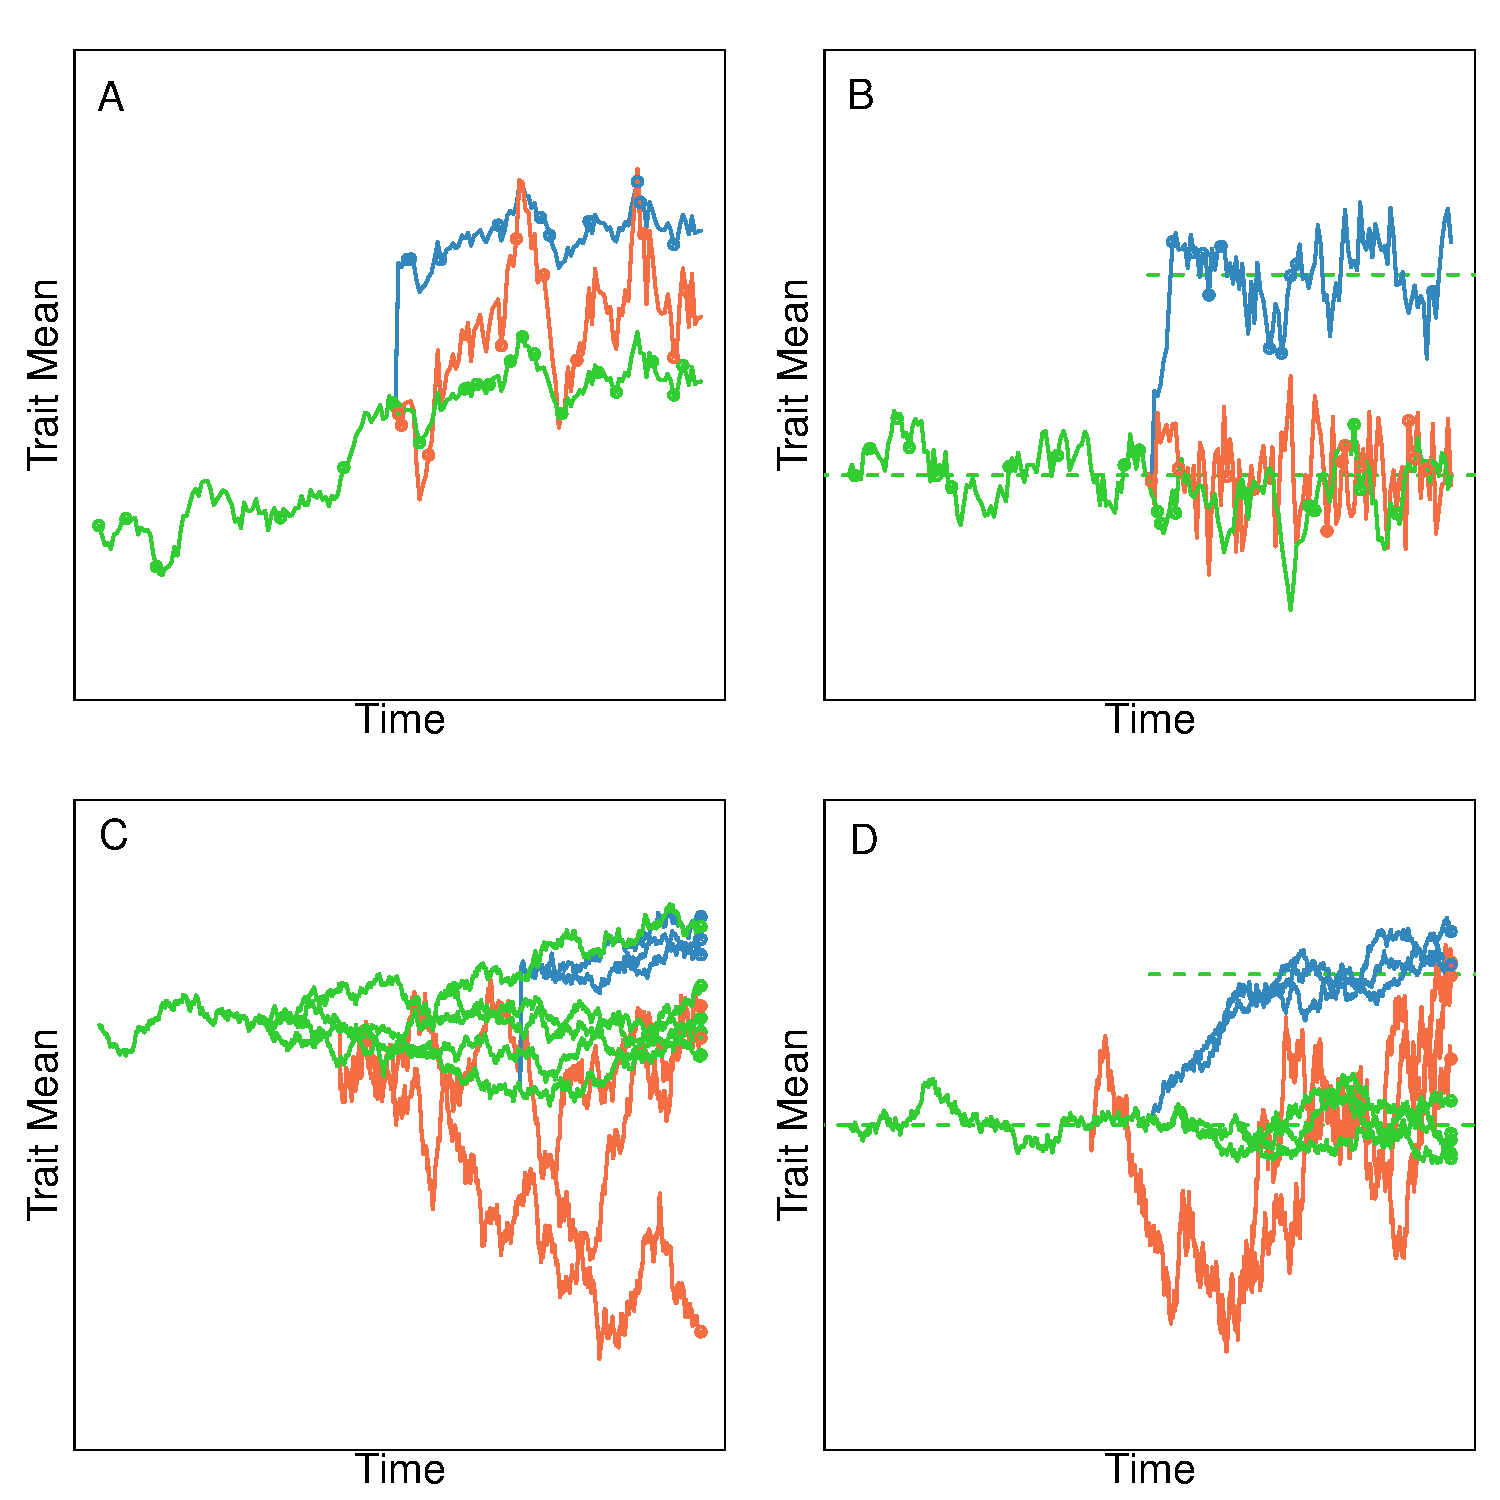
\includegraphics[width=\textwidth]{figs/Pennell_TREE-fig-box1}
\caption[Trait data simulated under alternative models]{Simulated datasets for different models of trait evolution from fossil time--series (A, B) and phylogenetic comparative data (C, D) under Brownian motion models (A, C) and Ornstein--Uhlenbeck models (B, D). Green lines are simulated as constant rate BM and OU processes, with circles indicating sampled data. Blue lines are discontinuous processes in which a burst of evolution occurs in the form of a single displacement (for BM models) or a walk to a new optimum ($\theta_2$) for OU models. However, all other parameters are kept constant. By contrast, red lines are models in which rate parameters ($\sigma^2$ and $\alpha$ for BM and OU models, respectively) shift to higher values and remain constant thereafter, but are not burst--like (no shift in the expected value of the process).  
}
\label{fig:pe-box1}
\end{figure}

BM models predict that divergence can increase without bounds, which is unrealistic under adaptive scenarios of trait evolution or under models of stasis, where traits are expected to evolve around adaptive optima. A simple extension of a BM model is an Ornstein-Uhlenbeck (OU) model of trait evolution. The per unit time change in mean phenotype under this model is:
\begin{equation}
\Delta \bar{z} = -\alpha(\bar{z}-\theta)+\sigma dW
\end{equation}
where $\sigma dW$ is identical to a BM process and contributes stochastically to divergence,  $\theta$ is the optimum trait value, and $\alpha$ is a ``pull'' parameter that governs how strongly the population mean is pulled toward $\theta$. Thus, divergence is a balance between the stochastic diffusion parameter ($\sigma^2$) and the deterministic pull parameter ($\alpha$) toward the optimum value ($\theta$) (Figure \ref{fig:pe-box1}). As with BM models, discontinuous OU models can allow for shifts in rate parameters ($\alpha$, $\sigma^2$), which has been implemented in a phylogenetic context \citep{Beaulieu2012}. Rapid shifts in optima are more naturally included in OU models via shifts in the $\theta$ parameter, and have been used extensively in phylogenetic comparative methods \citep{Hansen1997, ButlerKing2004, Beaulieu2012}. Population trait means approach a new optimum at a rate proportional to the strength of $\alpha$. Models with alternative patterns of selective regimes can then be compared via model selection techniques to evaluate adaptive hypotheses \citep{ButlerKing2004}. OU models have proven to be very useful for inferring various processes using both phylogenetic comparative \citep{Hansen2008, Mahler2013Science} and paleontological \citep{Hunt2008, Reitan2012} data.


\section{Box 2: An example of how PE can mislead inferences}
From a historical perspective, it is undoubtedly accurate that numerous comparative methods owe their genesis to the framework of PE. However, the temptation to frame these methods as tests of PE is, in our opinion, unwarranted. For example, \citet{Webster2003} developed a method to correlate the total genetic distance between the root and the tip of the tree (hereafter, the path length) with the number of nodes along that path (Figure \ref{fig:pe-box2}). A significant correlation between path length and the number of nodes rejects constant-rate gradualism in molecular evolution, purportedly in favor of a PE model. This correlation has been repeatedly demonstrated in a variety of datasets in traits ranging from molecular sequences to human languages (\citealt{Webster2003, Pagel2006, Atkinson2008, Lanfear2010}; but see \citealt{Goldie2011}).

\begin{figure}[p]
\centering
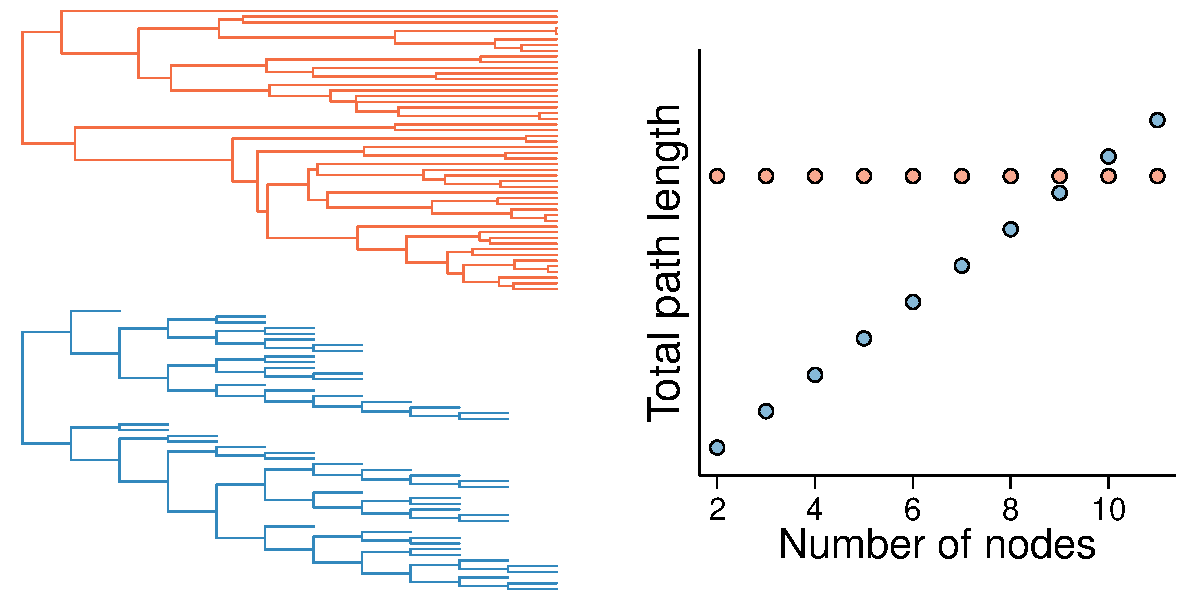
\includegraphics[width=\textwidth]{figs/Pennell_TREE-fig-box2}
\caption[Correlations between evolutionary divergence and speciation rates]{Illustration of a method for correlating evolutionary divergence with speciation. Branch lengths for both phylogenies are in units of evolutionary change. The total path length from the root of the tree to the tips is plotted against the total number of nodes along that path. A positive correlation (blue) is indicative of a relationship between the number of speciation events and evolutionary change, while under constant-rate gradualism no such relationship exists (red). Adapted from \citep{Pagel2006}.}
\label{fig:pe-box2}
\end{figure} 

However, to what extent is there evidence in these cases for PE? We argue: very little. Eldredge and Gould \citep{EldredgeGould1972} hypothesized that allopatric speciation causes pulsed phenotypic divergence. However, the direction of causality can just as easily be reversed. Genetic divergence is expected to promote speciation under many models of speciation \citep{Nosil2012}. Alternatively, divergence and speciation may result indirectly from causal links with a third factor, such as shorter generation times, higher fecundity, or increased genetic variation, to name a few \citep{Goldie2011}. Furthermore, trait evolution need not be pulsed for a positive correlation to exist. This effect was demonstrated by Rabosky \citep{Rabosky2012}, who showed that correlations between path length and speciation are expected whenever trait evolutionary rates are correlated with rates of speciation, even under purely gradual models. 

Finally, trait change may not be correlated with speciation at all, but instead be correlated with extinction rates.  This may occur, for example, if higher evolvability decreases extinction risk \citep{Lanfear2010}. It is certainly a worthwhile avenue of research to establish a correlation between diversification and trait evolutionary rates, but the available tests demonstrate nothing about whether or not trait evolution is pulsed, whether trait change accumulates anagenetically or cladogenetically or the direction of causality. Taking the ``off-the-shelf'' interpretation of these macroevolutionary patterns in the form of PE only obfuscates understanding, and worse, could lead to recapitulating four decades worth of often unproductive and contentious debates. Instead, we argue that we should focus on inferences that may be effectively tested using our available statistical tools. These tools should be integrated with more narrowly--defined theories that are free of the unwanted assumptions of PE.  

\section{Box 3: Modeling species selection and cladogenetic change on phylogenies}

In a ground-breaking paper, Maddison and colleagues \citep{Maddison2007} developed a statistical framework that has opened up investigation into two major components of PE--the influence of traits on diversification \citep[``species selection'', \textit{sensu}][]{CoyneOrr, RaboskyMcCune2010} and cladogenetic character change. The premise of the approach is that instead of specifying a full likelihood of the model, one need only to describe the probabilities of all possible events that could occur in a very short time interval, $\Delta t$, solve a differential equation and then use numerical integration to evaluate the likelihood of the model given the phylogeny and trait data at the tips (see \citealt{Maddison2007}, for full details). The initial model considered by \citet{Maddison2007} was the \textsc{bisse} model in which different states for a single character resulted in different diversification rates.

Consider that lineage diversification can be modeled by a birth-death process \citep{Kendall1948}, in which there is a constant rate of speciation $\lambda$ and extinction $\mu$ across the clade. Lineages with a trait in state $0$ diversify at rates $\lambda_0$ and $\mu_0$ and lineages in state $1$ diversify at rates $\lambda_1$ and $\mu_1$. Transitions (anagenetic evolution) between states $0 \rightarrow 1$ occur at rate $q_{01}$ and transitions from $1 \rightarrow 0$ occur at rate $q_{10}$. The probabilities of all possible events that can occur during $\Delta t$ can be described as a set of differential equations. One can then use the integration machinery, as described in \citet{Maddison2007}, to simultaneously estimate all parameters using either maximum likelihood or Bayesian inference to test for a statistical difference between $\lambda_{0}$ and $\lambda_{1}$ (or between $\mu_0$ and $\mu_1$) in order to infer the strength of species selection.

The \textsc{bisse} model was extended by \citet{MagnusonFord2012} (\textsc{bisse-ness}) to allow for the possibility of character transitions at speciation (cladogenetic change). (An identical model was independently derived by \citealt{Goldberg2012}, and related approaches were also developed by \citealt{Bokma2002, Bokma2008, Bokma2010}.) 

%\begin{figure}[p]
%\centering
%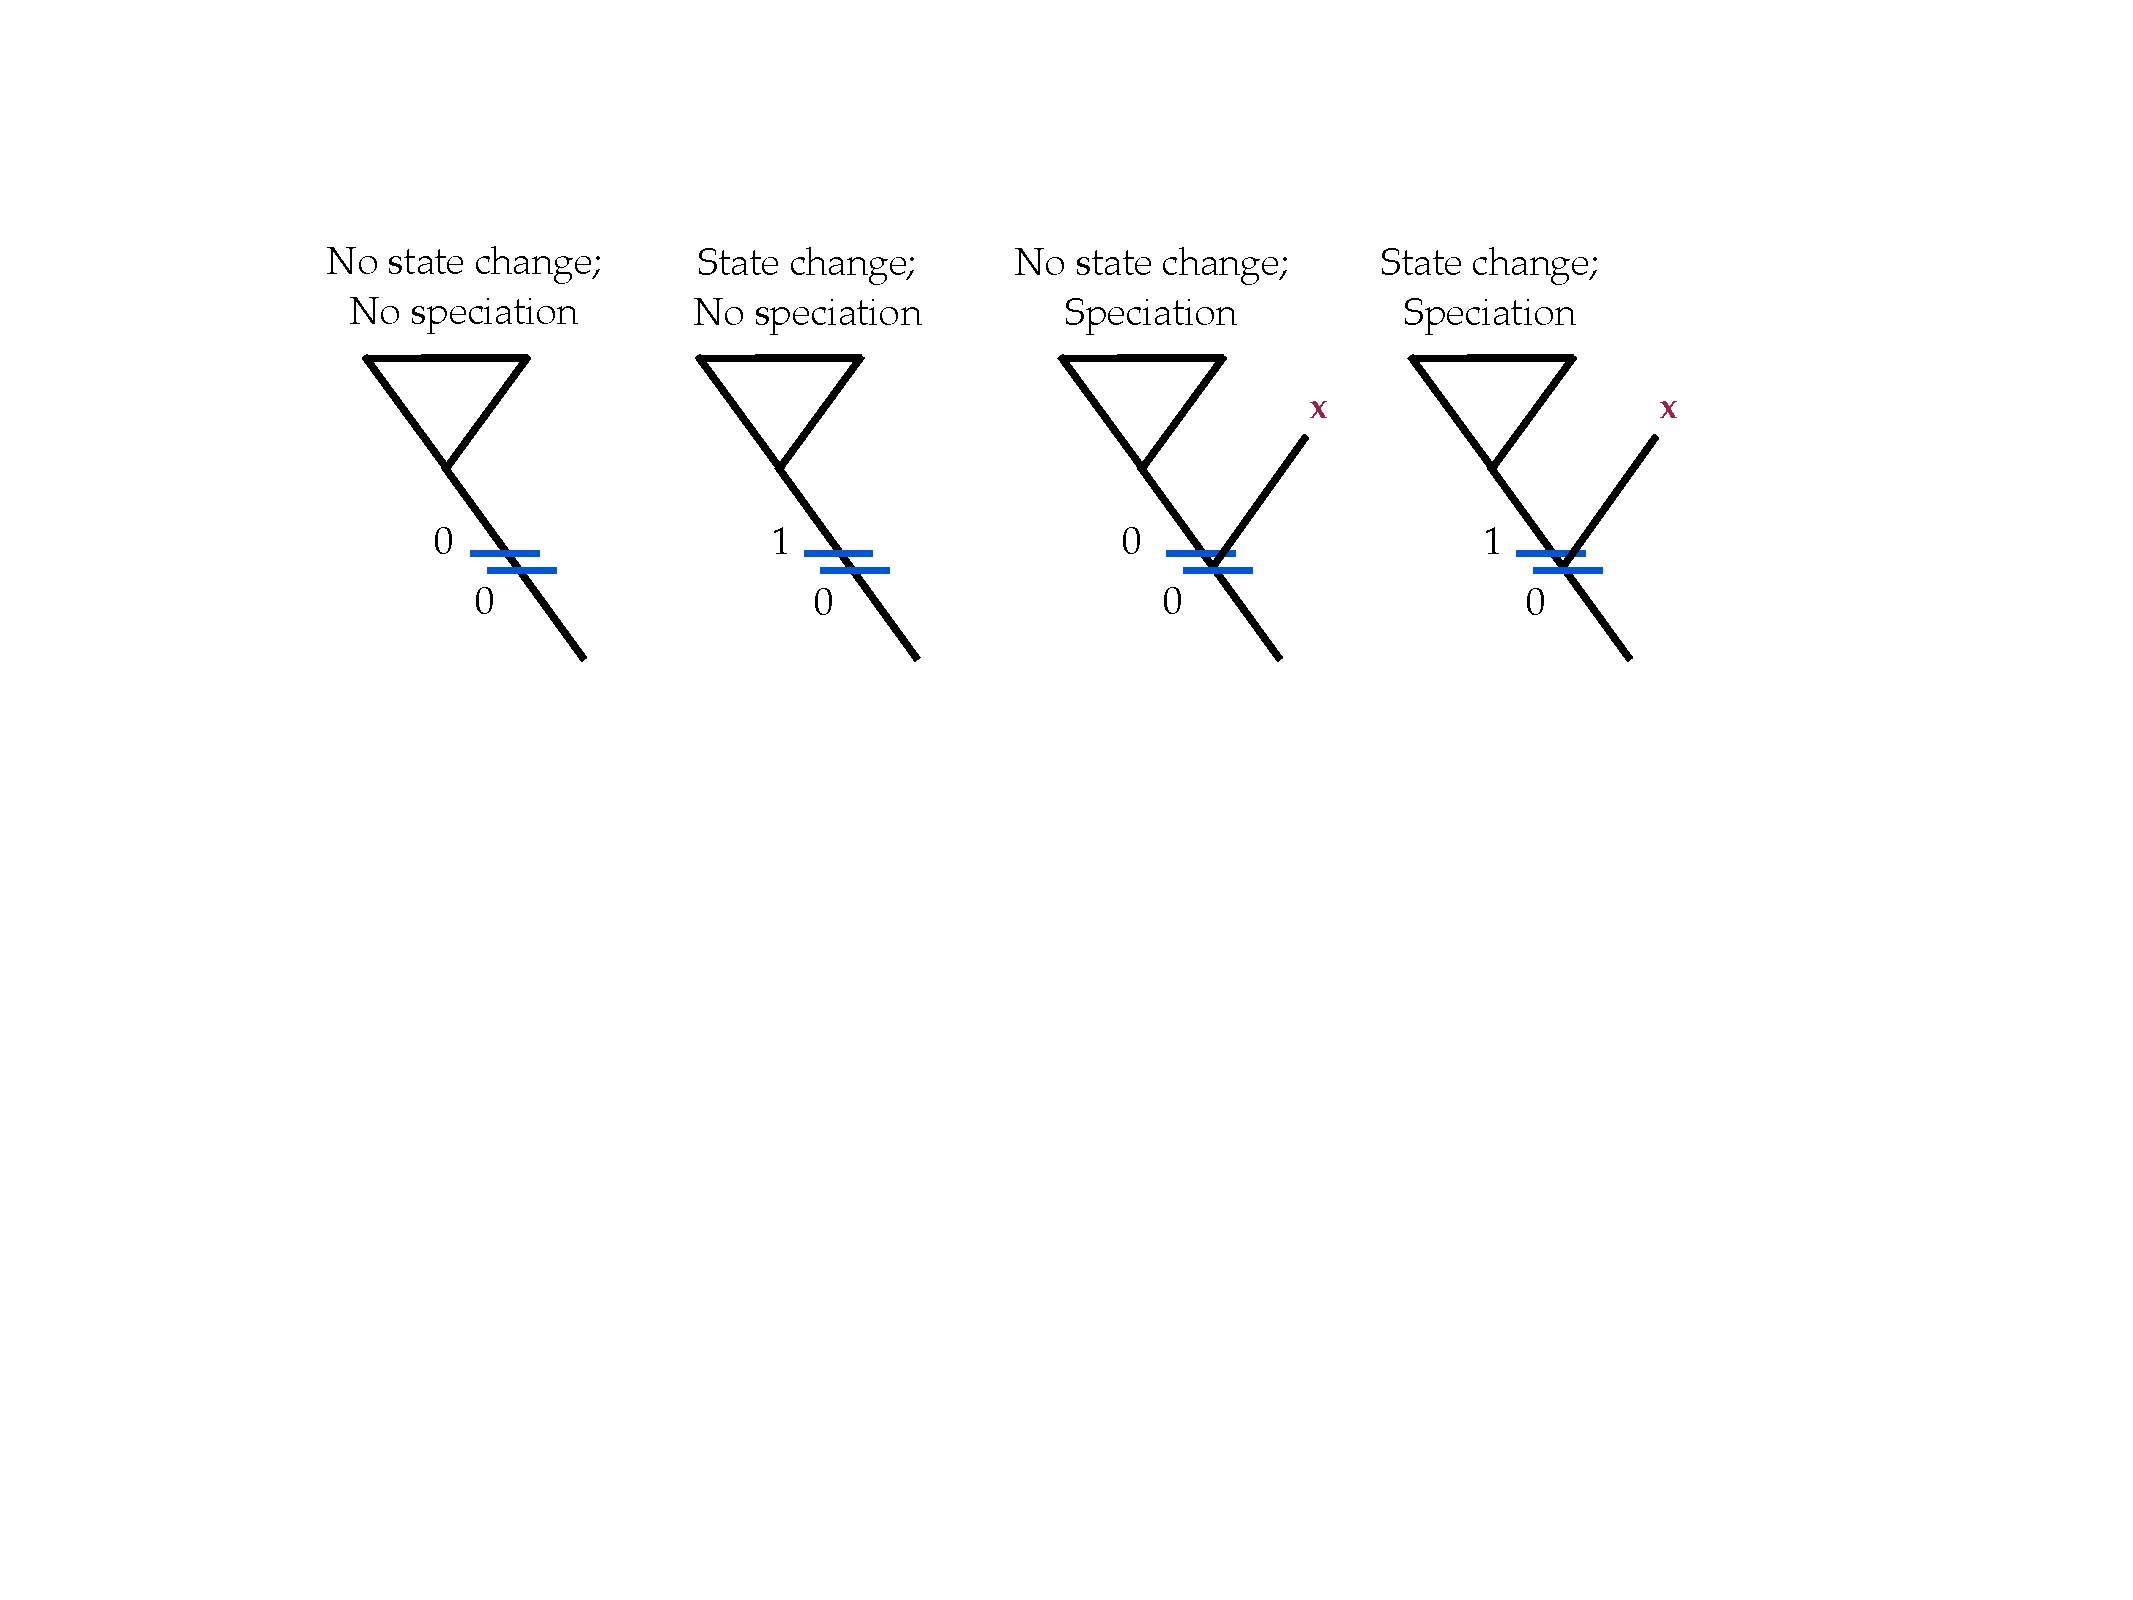
\includegraphics[width=\textwidth]{figs/Pennell_TREE-fig-box3}
%\caption[Illustration of BiSSE model]{A conceptual figure demonstrating how the BiSSE/BiSSE--ness model simultaneously model species selection and trait change. The four trees depict four possible events that could occur during a short time interval ($\Delta t$; the area between the two blue bars) along a given branch: no events happen; the trait changes; speciation occurs; both speciation and trait change occur. (These do not depict all possible scenarios.) If each event can be assigned a probability of occuring over $\Delta t$, one can derive differential equations describing the entire model and use numerical integration to calculate the likelihood of the model given a phylogenetic tree and trait data at the tips. Adapted from \citet{Maddison2007}.}
%\label{fig:pe-box3}
%\end{figure}

In addition to the 6 parameters of the BiSSE model ($\lambda_0, \lambda_1, \mu_0, \mu_1, q_{01}, q_{10}$), their model includes the probabilities of a change occuring at a speciation event ($p_{0c}$ and $p_{1c}$, for the two states, respectively) as well as the probabilities that the character changes are asymmetrical, where the change only occurs in one of the two daughter lineages, $p_{0a}$ and $p_{0b}$ (often referred to as ``budding cladogenesis'' in the paleobiological literature). This allows one to simultaneously evaluate the importance of species selection as well as the relative importance of cladogenetic versus anagenetic change. This model also highlights the general message of our paper; the questions can be evaluated independently of each other if parameter sets are constrained:

\begin{tabular}{ l c r }
  $\lambda_0 = \lambda_1, \mu_0 = \mu_1$ & Estimate cladogenetic and anagenetic rates only \\
  $q_{01}, q_{10} = \text{0}$ & Estimate species selection with only cladogenetic change \\
  $p_{0c}, p_{1c}, p_{0a}, p_{1a} = \text{0}$ & Estimate species selection with only anagenetic change\\
\end{tabular}\\

thus making it an excellent statistical framework, though certainly not the only one, for evaluating the questions associated with PE.


%%% Local Variables:
%%% TeX-master: "thesis"
%%% TeX-PDF-mode: t
%%% End:
